\documentclass[10pt,conference]{IEEEtran}
\IEEEoverridecommandlockouts
% The preceding line is only needed to identify funding in the first footnote. If that is unneeded, please comment it out.
\usepackage{cite}
\usepackage{amsmath,amssymb,amsfonts}
\usepackage{algorithmic}
\usepackage{graphicx}
\usepackage{textcomp}
\usepackage{xcolor}

\usepackage{hyperref}


\usepackage{url}
% kentHarvard requires natbib
\usepackage{natbib}
% add line numbers
% TODO: remove line numbers and run minted for release
% \usepackage{minted}
\usepackage{etoolbox}
\makeatletter
\patchcmd{\@verbatim}
{\verbatim@font}
{\verbatim@font\scriptsize}
{}{}
\makeatother

\usepackage{tikz}
\usetikzlibrary{shapes,arrows}

% Define block styles
\tikzstyle{decision} = [diamond, draw, fill=blue!20, 
    text width=4.5em, text badly centered, node distance=3cm, inner sep=0pt]
\tikzstyle{block} = [rectangle, draw, fill=blue!20, 
    text width=5em, text centered, rounded corners, minimum height=4em]
\tikzstyle{line} = [draw, -latex']
\tikzstyle{cloud} = [draw, ellipse,fill=red!20, node distance=3cm,
    minimum height=2em]


% \usepackage{lineno}
% \linenumbers
% \definecolor{periwinkle}{rgb}{0.8, 0.8, 1.0}
% \renewcommand{\linenumberfont}{\normalfont\bfseries\small\color{periwinkle}}
\usepackage{todonotes}

\usepackage{collab}  % [hideall]
\collabAuthor{sm}{red}{Stefan}
\collabAuthor{jl}{blue}{Joe}


\usepackage[autostyle]{csquotes}

\setcitestyle{numbers}
\setcitestyle{square}
\def\BibTeX{{\rm B\kern-.05em{\sc i\kern-.025em b}\kern-.08em
    T\kern-.1667em\lower.7ex\hbox{E}\kern-.125emX}}

\begin{document}

\title{Usage and Structure of Continuous Integration as Configuration?}

% \author{\IEEEauthorblockN{1\textsuperscript{st} Given Name Surname}
% \IEEEauthorblockA{\textit{dept. name of organization (of Aff.)} \\
% \textit{name of organization (of Aff.)}\\
% City, Country \\
% email address or ORCID}
% \and
% \IEEEauthorblockN{2\textsuperscript{nd} Given Name Surname}
% \IEEEauthorblockA{\textit{dept. name of organization (of Aff.)} \\
% \textit{name of organization (of Aff.)}\\
% City, Country \\
% email address or ORCID}
% \and
% \IEEEauthorblockN{3\textsuperscript{rd} Given Name Surname}
% \IEEEauthorblockA{\textit{dept. name of organization (of Aff.)} \\
% \textit{name of organization (of Aff.)}\\
% City, Country \\
% email address or ORCID}
% }

\maketitle           %% restore the layout


% This is good but the last conclusion bit needs work on
% I thin that it should be a lot better when RQ3.5 is written up to show more on CI usage as we can go 70% of projects contributed to in the last year use CI in comparison to only 50% of projects that were contributed in the last 2 years
% NOTE: have to careful when doing time comparisons as currently I am doing it as time windows so "last 2 years" doesn't work as that is 2 years of data not 1 year

\begin{abstract}
\sm{title needs to reflect the center piece of the paper.
How about something like:
Usage of Continuous Integration Services on GitHub
}

Continuous integration (CI) is widely popular
for instance as support for fast-paced development cycle.
\sm{do we want to frame the paper around a reproduction of the earlier study?
Since this seems to be the strongest part, I would start out with this.
Pose the question of whether things have changed since people looked at it last.}
This paper investigates how CI is currently used by projects on GitHub.
To our knowledge, the last major study was in 2016
by \citeauthor{Hilton2016}\citep{Hilton2016}
and we want to see how things changed in the last 5 years.
% In doing so compared our results against \citet{Hilton2016} work to see if their has been a increase in usage.

We analyze 94,379 open source projects from GitHub % to answer these questions.
to understand how CI is used based on the corresponding configuration files.

% Most CI is done automatically using a service which runs based off configuration.
% Our major questions is how much is CI actually being used?
%As well as how are these files being structured?   
We found a shift in CI services being used.\sm{can we give an example here?
trying to summarize the results a little}
% and were able to get similar results to their study.
\sm{for the structure, I'd suggest to use something else than the comment bit}
% In terms of structure we found that configuration files are written with no comments normally. We suggest at the end further research is needed to get a better understanding of this growing field.

%% This is the old abstract, the system can be updated, we don't really need it here
% \jl{this is what I submitted last week as the abstract, it looks like we might be able to update it via the site}
% Continuous integration (CI) is becoming more popular as software development moves to an Agile fast paced development life cycle.
% This paper investigates how CI is currently used by projects on GitHub.
% To our knowledge, the last major study in 2016 by Michael Hilton and we want to see how things have changed over the last 5 years.
%
% We got 94,379 open source projects from GitHub to answer these questions.
% We found a shift in CI services being used in particular the rise of GitHubActions and we found similar usage numbers.
% Additionally, we looked at structure of CI configuration, we found that average configuration files remained small (under 100 lines) but over 50\%
% used external scripts for additional functionality. We suggest at the end further research is needed to get a better understanding of this growing field.

\end{abstract}



\section{Introduction}
\label{Introduction}

Continuous integration (CI) is becoming more popular over the last few years. This can be seen by how major version control hosting services GitHub, Bitbucket and Gitlab have all released CI products or have been improving their CI products. In terms of research, Infrastructure as Code in \citet{Rahman2019} which does a systematic mapping of research in that area. For Continuous Integration with \citet{Shahin2017} which does another systematic review on how it is used. These two papers demonstrate some of breadth of research that has taken place. In addition you have papers like Google's Innovation Factory: Testing, Culture, and Infrastructure \citet{Copeland2010} which demonstrate some of the depth that the papers go into.

Continuous Integration is a process of automatically compiling, running tests and checking that the product works. This is can be combined with Continuous Delivery where the product is deployed or released after it has gone through successfully CI. 

This can get complicated quickly therefore Configuration as Code (or Infrastructure as Code) is used to configure it. The main kind of configuration format used for this is Yaml followed by Xml and Java based scripting formats.


In order to look at our first theme CI usage we looked at In Usage, Costs, and Benefits of Continuous Integration Open-Source Projects \cite{Hilton2016}. They looked closely at the usage of CI as well. As we are looking at CI usage as well we are going answer the first three questions from their theme \enquote{Usage of CI}. 
\begin{itemize}
  \item \textbf{RQ1} What percentage of open-source projects use CI?
  \item \textbf{RQ2} What is the breakdown of different CI services?
  \item \textbf{RQ3} Do certain types of projects use CI more than others?
  \item \textbf{RQ 3.5} Do more recently contributed projects use CI?
\end{itemize}

We will be using doing a comparison with our corpus against theirs in order to work out what has changed over the last 4 years. 

It would have been really interesting to do a full in depth analysis of each CI configuration format like \citet{Gallaba2018} does for Travis. However we can look at the general structure of all the CI configuration files allowing for comparisons to be made between configuration files. As that will allow comparisons to be made more easily otherwise comparing very specific features would have been harder.
\begin{itemize}
  % Could have "How are configuration files broken down?"
  % syntax errors, line counts, comment analysis all available but it's not quite coherrent
  % so combining into one and maybe even deleting script usage might be for the best.... or just adding it in there....
  % as it's about quality not quanity and there is a strict limit on words
  \item \textbf{RQ4} What are the common errors when loading yaml configuration?
  \item \textbf{RQ5} How are comments used in the configuration?
  \item \textbf{RQ6} How are external scripts used within the configuration?
\end{itemize}

\section{Related Works}
\vspace*{-0.05in}
\subsection{Continuous Integration}
\vspace*{-0.05in}

Continuous Integration is frequently submitting work normally tied into a feedback loop. For example using version control and committing changes daily. For each changed committed a server builds and tests the changes informing you of status of those changes. As well as providing a build which is typically a binary executable of code that can then be saved if necessary. In doing you can reduce the chances of facing the situation off \enquote{It works on my machine...}. As the building and packaging of the code is done on a server to make sure everything integrates.

An early definition of CI was written up and then updated later by Martin Fowler \cite{CI2010_MartinFowler}. A key part of the CI is that allows teams to work on the same code base which without CI could easily lead to integration bugs and broken builds. 

To enable to this to happen automation needs to put in place for build, testing and other aspects of the integration process in order that a clear piece of feedback (yes or no) can be given about the status of the build. If done with a version control system, if the same commit is built twice (so no changes have happened) it is vital that it produces the same result. Otherwise it is hard for a team to be able to depend on CI result if they are getting flakey test results or flakey build results.

\vspace*{-0.05in}
\subsection{Usage of Continuous Integration}
\vspace*{-0.05in}

The actual usage of CI was looked at by \cite{Hilton2016}. In this they use three source of information GitHub repositories, Travis builds and a survey. The impact of CI usage on GitHub was looked as well in \citet{Vasilescu2015}. The key difference is that we will be looking at the configuration alongside the CI usage and leaving impact of CI on the project to further research or current existing research. In analysing that data they found that \enquote{The trends that we discovered point to an expected growth of CI. In the future, CI will have an even greater influence than it has today.} As we are looking at the same question we will use four of the research questions out of the fourteen (\ref{section:RQ1}, \ref{section:RQ2}, \ref{section:RQ3}). In order to see what difference four years has made to the growth of usage of CI.

In addition to comparing to the previous study we will also look into how CI usage changed over the years. \todo{basically want to expand on \ref{section:RQ3}might also move some stuff out of RQ3 to make it more of a straight up comparison}

\vspace*{-0.05in}
\subsection{configuration as code}
\vspace*{-0.05in}

Configuration as code or Infrastructure as Code has been an increasing area of research over the last few years. There seems to be slightly more research in infrastructure as code, for example see \citet{Rahman2019}. The has been a focus on Puppet and Chef, for example \citet{Sharma2016} looked at code quality by the measure of \enquote{code smell} of Puppet code. This tackles the problem by defining by best practices and analyzing the code against that. In the case of \citet{Cito2017} it uses the docker linter in order to be able to analyse the files. 
For the CI systems we pick we will look into the tooling around that to aid the analysis.


\section{Methodology}
\label{methodology}
% here we want to describe why we went with GitHub over GhTorrent 
In order to answer the research questions we needed to find projects for CI configuration files. This is because we needed to get the contents of the configuration in order to analyse the structure of it. We chose to scrape GitHub via their API as it was easy to setup and test whether or not it was working as there is a one-to-one mapping between the API and user interface. Using Ghtorrent \citet{GhTorrent2020} it may have been easier to gather more data because the rate limiting wasn't as strict. Yet harder to test whether or not it is working. Therefore we decide to use the GitHub API as the source for our corpus.

\begin{figure}[!htbp]
  \centering
  \begin{minipage}{.48\textwidth}
    \centering
    \includegraphics[scale=0.5]{repository file system.png}
    
    \caption[alt text]{Example GitHub repository that has multiple configuration types in it \cite{GithubRepoExample}. (This is an old repository that was reused in order to test out the scraper)}
    \label{image_example_repo}
  \end{minipage}%
  \hfill
  \begin{minipage}{.48\textwidth}
    \begin{verbatim}
      PATHS = {
        "travis": "travis",
        "gitlab": "gitlab-ci",
        "azure": "azure-pipelines",
        "appVeyor": "appveyor",
        "drone": "drone",
    
        "jenkinsPipeline": "jenkinsfile",
        
        "teamcity": ".teamcity/",
    
    
        "github": ".github/workflows/",
        "circleci": ".circleci/",
        "semaphore": ".semaphore/",
        "buildkite": ".buildkite/"
    }
    PATHS_MULTIPLE = ["github", "circleci", "semaphore",
     "teamcity", "buildkite"]
    NONE_YAML = ["jenkinsPipeline", "teamcity"]
    \end{verbatim}
    \caption{Python configuration file used to specify what types of configuration to search for. The key specifies the name of the configuration and the value is the location in the repository the config should be found.}
  \end{minipage}
\end{figure}

We chose to use a config file to specify which CI systems configuration files we would look for. If it was a directory then it would get all \enquote{.yaml} or \enquote{.yml} along with any Teamcity \enquote{.kts} and \enquote{.xml} files. However the script did not look into any of the sub directories which might be the cause for the low number of Teamcity configuration files found. In the case that it was a file that was on the top level directory we matched it with the lowercase file name we found against the query.

In terms of which configuration files to pick we based our list from GitHub Welcomes all CI Tools blog post in 2017 \cite{Github2017}. In addition we added GitHub Actions and Azure Pipelines to the list as they are new and potentially popular systems. 


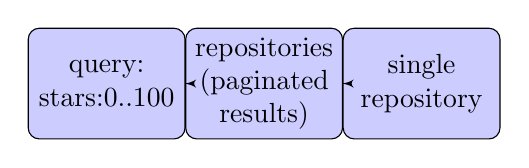
\begin{tikzpicture}[node distance = 2cm, auto]
  % Place nodes
  \node [block] (init) {query: stars:0..100};
  \node [block, right of=init] (repos) {repositories (paginated results)};
  \node [block, right of=repos] (repo) {single repository};
  % Draw edges
  \path [line] (init) -- (repos);
  \path [line] (repos) -- (repo);
\end{tikzpicture}

\begin{figure}[!t]
  \centering
  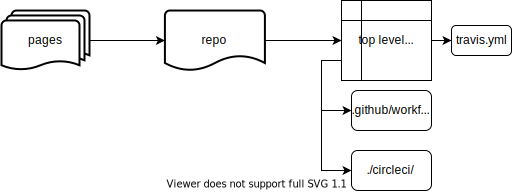
\includegraphics[width=2.5in]{methadology diagram.pdf}
  
  \caption[alt text]{Diagram of the process used to search for projects with CI files in them}
  \label{image_methadolgoy_diagram}
\end{figure}

As can be seen in Figure \ref{image_methadolgoy_diagram} a query based on the number of stars a project has on GitHub. This is because we need a way of getting a large sample from GitHub without introducing too much bais into the sample. That is not too say that our method is perfect but it provides an easy way to get a large sample that includes projects with and without CI.
Another potential solution would have been to use the \enquote{filename:travis.yaml} search API. However this did not provide information about which projects did not use CI. Additionally for one unique search their can only be 1000 results returned by the GitHub API. To mitigate that limit we search based stars as we did do a search for a 1000 results per star count. The limitation of this though was that there will be over a 1000 repositories that have 0 to 500 or even 500 to 501 stars. That means it is a sample that represents some of the population but not a sample of all CI files on GitHub. 

As the config could have mistakes in it or we missed out a major CI system. We also saved the ReadMe.md when we scraped each project. A Readme.md is used to describe a project and will be displayed on GitHub at the bottom of the root directory. As can be seen in Figure \ref{ExampleGitHubReadme} some ReadMe's have a label and/or links to the CI system used for that project. Therefore we also saved that data when we scraped a project. 

\begin{figure}[!t]
  \centering
  \includegraphics[scale=0.5, width=2.5in]{2020-01-30-08-29-04.png}
  
  \caption[alt text]{Example of CI tag for GitHub ReadMe \cite{GithubReadMeExample}}
  \label{ExampleGitHubReadme}
\end{figure}

We ended up with searching for the following CI systems: Travis, Gitlab, Azure, App Veyor, Drone, Jenkins, GitHub, Circleci, Semaphore, Teamcity and Buildkite. 

We excluded Wrecker from the search because they represented a very small number of projects in comparison to the other projects. As it seems since the GitHub survey in 2017 they got bought by Oracle and from doing a search on GitHub for what we think based on the docs \cite{WreckerDocs} and \cite{WreckerOpenSourceGithubSearch} for their configuration file naming convention. We were only able to find 20 results so did not include in the scraping script to speed up the process of searching for the other configuration file formats. Despite it being used in the \citet{Hilton2016} paper.

Along with information of what CI is being used for a project we also gathered metadata about the project. The available metadata through the API is largely what can been seen on a repository for example in Figure \ref{ExampleGitHubMetaData}. We have the star count which is an indication how popular a project is as users can star projects that they like \citet{Borges2016}. Then we have watchers which is users that have subscribed to the project to get notifications about the project. 

\begin{figure}[h]
  \centering
  \includegraphics[scale=0.5, width=2.5in]{readme metadata example.png}
  \caption[alt text]{Example GitHub project description and metadata\cite{GithubMetaDataExample}. The orange sections sections highlighted are the metadata that we scraped.}
  \label{ExampleGitHubMetaData}
\end{figure}

\vspace*{-0.05in}
\subsection{Data corpus}
\label{section:corpus}
\vspace*{-0.05in}
This all produced a sample of 32,660 projects from open source projects on GitHub. As can be seen in Figure \ref{graph_scatter_stars_vs_subs} we weren't able to scrape the whole star count range easily. This is because the script would crash when GitHub gave a 500 error code at us randomly. Along with empty repositories initially causing a problem. In order to mitigate the damage of this the scraper would create a new Comma Separated Value (csv) file search e.g. one for stars:0..1 and another for stars:1..2. As all the csv file contained the same header we ran a script to combine all together at the end. Making sure to remove any duplicates by filtering on the GitHub project id.

\begin{figure}[!htbp]
  \centering
  \includegraphics[width=2.5in]{../src/results/sub vs stars.pdf}
  \caption[alt text]{GitHub stars against subscribers}
  \label{graph_scatter_stars_vs_subs}
\end{figure}

\vspace*{-0.05in}
\subsection{Comparison corpus info}
\label{section:HiltonComaprisonCoprusTHing}
\vspace*{-0.05in}
In \citet{Hilton2016} paper they use a similar method of using the GitHub API in order to create their corpus. Additionally they contacted Cloud Bees \citet{CloudBees2020} to get a list of all open source projects that used their services. This helped them not to miss out on projects that they would otherwise missed out on. They kindly gave a copy of their final corpus. 

However it does contain the data on the Cloud Bees projects which is 223 projects. As far as we can tell this only affects the comparison done in RQ2 \ref{section:RQ2}. Additionally we found slight discrepancies between the paper and corpus in RQ1, RQ2 and RQ3, these being mainly mainly just a few numbers off in a few places. In order to do comparisons well and to keep it consistent we will be basing all our comparisons from the corpus. As the discrepancies are small we will still be using the conclusions from the paper where possible.  

In order to get a better understanding of the results of the methodologies chosen in both cases. We created two histograms to showing the density by the stars of the spread of data using the Sturge's rule (Figure \ref{graph:hist}). As we expected both corpses are skewed to the left. They use a logarithmic scale and initially it can look like there more data in 2020 corpus. However it is just more spread over the stars and potentially had a larger search range used. In Figure \ref{graph:hist2016} there is data after 40,000 stars potentially this could be down to the search method used or that most projects weren't dispersed over so many stars on GitHub.   

\begin{figure}[!htbp]
  \centering
  \begin{minipage}{.48\textwidth}
    \centering
    \includegraphics[width=2.5in]{../src/results/density_2016.pdf}
    \caption[]{2016 corpus}
    \label{graph:hist2016}
  \end{minipage}
  \begin{minipage}{.48\textwidth}
    \centering
  \includegraphics[width=2.5in]{../src/results/density_2020.pdf}
  \caption[]{2020 corpus}
  \label{graph:hist2020}
  \end{minipage}
  \caption[]{Histogram showing the density for both corpses via the stars of the projects. They are both skewed towards to the lower star count projects. }
  \label{graph:hist}

\end{figure}



% ------------------------------------------------------------------------------------------------------------------------------------

\pagebreak
\section{Usage of CI}

\vspace*{-0.05in}
\subsection{\textbf{RQ1}: What percentage of open-source projects use CI?}
\label{section:RQ1}
\vspace*{-0.05in}

Out of the 94,379 projects 42.25\% of them had CI configuration files in them indicating that they used CI in our dataset. 

\begin{table}[!ht]
    \begin{tabular}{l|l|l|l|l|}
    \cline{2-5}
                                                        & \multicolumn{2}{c|}{\textbf{2016}} & \multicolumn{2}{c|}{\textbf{2020}} \\ \cline{2-5} 
                                                        & count      & percentage             & count         & percentage         \\ \hline
    \multicolumn{1}{|l|}{\textbf{CI}}                   & 13,752     & 39.81\%               & 37,417        & 39.65\%            \\ \hline
    \multicolumn{1}{|l|}{\textbf{ReadMe has CI status}} & \multicolumn{2}{c|}{n/a}           & 2462          & 2.61\%             \\ \hline
    \multicolumn{1}{|l|}{\textbf{Multiple CI}}          & \multicolumn{2}{c|}{n/a}           & 1764          & 14.07\%            \\ \hline
    \multicolumn{1}{|l|}{\textbf{No CI found}}          & 20,792     & 60.19\%               & 54,500        & 57.75\%            \\ \hline
    \multicolumn{1}{|l|}{\textbf{Total}}                & \multicolumn{2}{c|}{34,544}        & \multicolumn{2}{c|}{94,379}             \\ \hline

    \end{tabular}
    \label{table:comparison_dataset}

    \caption{This table shows the comparison between the 2016 dataset which is\citet{Hilton2016} and our dataset labeled as 2020. For the CI usage in each dataset along with what percentage of projects contained multiple CI setups.}
\end{table}
% table references are not working because the table was being rendered below the reference.... ah! but it's fixed atm 
An interesting factor in Table \ref{table:comparison_dataset} is the percentage of that 38\% that has multiple CI in them. This is because configuration files can be used to CI or Continuous Deployment (CD) and some projects are run a monorepo which means that they have multiple projects inside them. Another simple explanation is that although the configuration is stored version control it just hasn't been deleted. 

We scraped the \enquote{ReadMe.md} files from the projects to check if they had a CI status label in them as shown in Figure \ref{ExampleGitHubReadme}. To do this we checked for \verb|alt="Build Status"|, \verb|alt=`Build Status'|, \verb|Status| and \verb|status| being in the file. Then if that same line of text contained a url specified by if contained \verb|http://| or \verb|https://| then we counted it as potentially being a project that used CI. In order to check the validity of this method we ran it on all projects that we had found configuration files for. We got 6782 (55.92\%) \todo{REDO with new data to get the stats to line up but only metha}projects with a ReadMe that had a CI status label that we could find. 
However this method is not perfect, for example \enquote{awesome-bootstrap-checkbox} by \enquote{flatlogic} \cite{GithubReadMeIncorrectFind} their ReadMe has the following line:
\begin{verbatim}
  [![Dependency Status]
  (https://img.shields.io/david/dev/flatlogic/awesome-bootstrap-checkbox.svg?branch=master&style=flat)
  ]
  (https://www.npmjs.com/package/awesome-bootstrap-checkbox) 
\end{verbatim}
This contains \verb|Status| and a url so we say it has got CI when the repository currently doesn't. Yet this is not the case for all of them as for example \enquote{SyncTrayzor} by \enquote{canton7} \cite{Male2020} uses AppVeyor but doesn't use a configuration file for it. Therefore we didn't find it as we searched for a configuration file only. 

The percentage of CI projects in 2016 was 39.81\%. If you look at Table 1 it shows that we got 42.25\% CI projects. This shows a slight increase in CI usage however if we look at just projects where we can confirm to have found CI it is very close still at 39.65\%. 

One possible reason could be because in RQ3 \ref{section:RQ3} it shows that the more popular a project the higher chance it has of using CI. Therefore as their sample contains a few more projects that are popular they could all be more likely to be using CI. However that is a weak tangent to make in order to full explain it.  

Another possible reason could be if you combined the \enquote{Found CI} and \enquote{ReadMe has CI status} results together for 2020 you would get 41.28\% which is shows that our sample is within the margins of the same results that of CI usage for 2016.

A further possible explanation GitHub's growth over the last 4 years (\citet{GithubOctoverseResults2016} to 2019 \citet{GithubOctoverseResults}) so that GitHub is now at 40 million active users. It means that there are more projects that are using CD setups for building their static sites and in general GitHub is being used for more things that wouldn't require CI.

We think that the last two factors are the most likely contributors to why there is less CI usage now. Another important interesting aspect is that despite GitHub growing so much the CI usage rate has stayed relatively the same. 



% --------------------------------------------------------------

\vspace*{-0.05in}
\subsection{\textbf{RQ2}: What CI systems are projects using?}
\label{section:RQ2}
\vspace*{-0.05in}
In Table \ref{table_config_types} we, like all other research, found that Travis is the most popular CI system in use. However over the last 4 years the \cite{Github2017} CircleCi has lost out on it's rough quarter that it owned in the market. Notably the rise of GitHub Actions seems to have taken second place in the market share even though it is still very young in comparison as it was officially released November 13th 2019 but had a closed beta since the summer of 2019. This might not be down to the CircleCi losing out on their existing share, but maybe due to the rise in CI usage on GitHub. As well as because we searched GitHub for projects GitHub's CI product would be popular on their platform.

\begin {table}[!htbp]

\caption{Configuration types spread}
\label{table_config_types}
\begin{tabular}{|l|r|l|}
\hline
{} &  config & percentage \\ \hline

Travis          &   10607 &        74\% \\ \hline
Github          &    2301 &        16\% \\ \hline
CircleCi        &    1109 &         8\% \\ \hline
Jenkins pipeline &     161 &         1\% \\ \hline
Drone           &      84 &         1\% \\ \hline
Buildkite       &      32 &         0\% \\ \hline
Teamcity        &       4 &         0\% \\ \hline
Semaphore       &       2 &         0\% \\ \hline
Azure pipeline           &       1 &         0\% \\ \hline

\end{tabular}
\end{table}


\begin{figure}[!htbp]
  \centering
  \begin{minipage}{.48\textwidth}
    \centering
    \includegraphics[width=2.5in]{../src/results/comparison_config_bar.pdf}
    \caption[]{2016 corpus}
    \label{graph:config_bar2016}
  \end{minipage}
  \begin{minipage}{.48\textwidth}
    \centering
  \includegraphics[width=2.5in]{../src/results/config-topn.pdf}
  \caption[]{2020 corpus}
  \label{graph:config_bar2020}
  \end{minipage}
  \caption[]{Percentage bar graph showing the usage of each CI service. The key difference is how CircleCI has got a lower rank. Due to rise of GitHub Actions which only open to closed beta in August 2019}
  \label{graph:config_bars}

\end{figure}

\todo[]{double check this paragraph!!}
Our sample size of repositories is 31,494 that as it is a representation of projects on GitHub so won't account for the whole of it. This means that although Wrecker had the smallest count of CI when researching of 20 projects. In Table \ref{table_config_types} we have configuration types that have lower counts. This is because that search for the 20 searched the whole of GitHub but the scraping was only able to do a small sample. Additionally there potentially could be faults in the scraping causing it show such low numbers for the last 3. 

% ------------------------------------------------------------------------------------------------------------------------------------
\vspace*{-0.05in}
\subsection{\textbf{RQ3}: Do certain types of projects use CI more than others?}  
\label{section:RQ3}
\vspace*{-0.05in}

In Figure \ref{fig:comparison_percentage_star_usage} shows all the CI projects sorted then grouped together per 540 projects. The number used to group the projects was chosen based off the average group size used when \citet{Hilton2016} conducted this question. Then in this case we choose to categories via star count for each project. 

\begin{figure}[!htbp]
  \centering
  \begin{minipage}{.48\textwidth}
    \centering
    \includegraphics[width=.9\textwidth]{../src/results/percentage sub with CI other paper source.pdf}
    \caption[]{2016 dataset}
    \label{fig:test1}
  \end{minipage}
  \begin{minipage}{.48\textwidth}
    \centering
    \includegraphics[width=.9\textwidth]{../src/results/percentage stars with CI.pdf}
    \caption{2020 dataset}
    \label{fig:test2}
  \end{minipage}%
  \hfill
  \caption{In Figure \ref{fig:test1} is the results from this research and in Figure \ref{fig:test2} is the results from \cite{Hilton2016}. The results show the percentage chance of CI usage depending on the number of stars a group of 540 projects has on average.}
  \label{fig:comparison_percentage_star_usage}
\end{figure}

In Figure \ref{fig:test1} and \ref{fig:test2} we are comparing whether or not in the last 4 years the number of stars increases the amount CI being used. It shows how the trend in the more popular the project by how you have more stars for a project increases the chances it uses CI has stayed the same. However the gradient of that trend which has changed to be slightly greater overall, yet not quite as sharp for the end of the graph, this is most likely because the 2016 dataset doesn't have as much data between 40000 and 90000 as seen in Figure \ref{graph:hist2016}.

\begin{figure}[!h]
  \centering
  % TODO: make this bigger when the time comes
  \includegraphics[width=.8\textwidth]{../src/results/percentage sub with CI.pdf}
  \caption{Subs graph}
  \label{graph_percentage_subs}
\end{figure}
Figure \ref{graph_percentage_subs} uses the same method as Figure \ref{fig:comparison_percentage_star_usage} except it does it based the number of subscribers. Subscribers are users on GitHub who want to keep update on the changes to a project. This could range from core team members working on the project to people that want to be notified about a new release. 
In looking at this metric the hypothesis was that it would have a sharper rise in percentage of projects using CI per subscriber. However that was not the case overall as the gradient is not as strong. There is no comparison to \cite{Hilton2016} because their final corpus does not contain the subscriber count for each project.

That gives us a good look at how projects can be viewed through GitHub's metadata. 


Next we turn to what kind of programming languages are being used for CI. Figure \ref{graph:programming_langs_count_ci} shows the  top 20 programming languages by count and we can see that Javascript is the most common kind of project by a considerable margins. This was to be expected as it ties in with GitHub's annual report \cite{GithubOctoverseResults} on the platform they reported that Javascript has been the most popular programing language for the last 5 years. The interesting part is that our sample matches the rise in Python over Java. This is despite the fact that they are using \enquote{unique contributors to public and private repositories tagged with the appropriate primary language} and we are using the count of projects by primary programming language tag. 

\begin{figure}[!h]
  \centering
  \includegraphics[width=.8\textwidth]{../src/results/languages-topn.pdf}
  \caption{Count of top 20 programming languages used by projects using CI}
  \label{graph:programming_langs_count_ci}
\end{figure}

In order to get a better idea of the breakdown of the effect programming languages have on CI usages we created Figure \ref{graph:scatter_langauges_CI}. This shows three pieces of information the percentage of CI usage on the y axis, average star count on the x axis and then number of projects using the language by the size of the dot. 

\begin{figure}[!h]
  \centering
  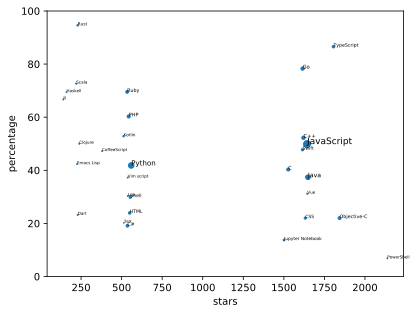
\includegraphics[width=.8\textwidth]{../src/results/languages-scatter-CI.pdf}
  \caption{Scatter graph showing the top 30 most used programming languages against how much they use CI. The key points are Rust, Typescript and Go being the top three programming in CI usage.}
  \label{graph:scatter_langauges_CI}
\end{figure}


The most striking part of Figure \ref{graph:scatter_langauges_CI} is the clear divide between different programing languages star count. The programming with the languages with the highest CI usage are Rust (94.6\%), Typescript (86.56\%) and Go (78.31\%). This is interesting in that they are all fairly \enquote{new programming languages} in comparison to the others in the graph. They are all languages which are developed and open source on GitHub. In terms of Rust and Go it could be down to their tooling that comes built in to the language as that would lead to implementing CI to be a lot easier. Typescript is more a special case as it is a subset of Javascript so uses `npm' to deal with dependency management which was some of the inspiration for Rust's tooling \citet{RustBlogCargo}. Older programming languages like Java and C\# both have tooling for dependency management but the chances that they use CI is much lower. Therefore an area for further research would be whether or not the use of \enquote{modern} dependency management systems increases the chance of CI.

\begin{figure}[!h]
  \centering
  \includegraphics[width=.8\textwidth]{../src/results/scatter.pdf}
  \caption{Scatter graph showing the top 30 most used programming languages against how much they use CI for \citet{Hilton2016} from 2016. In comparison to Figure \ref{graph:scatter_langauges_CI} the data is not as grouped as clearly by the star count. Rust, Typescript and then Scala have the highest programming CI usage.}
  \label{graph:scatter_langauges_CI_2016}
\end{figure}

In figure \ref{graph:scatter_langauges_CI_2016} it shows the sample from 2016 in comparison to \ref{graph:scatter_langauges_CI}. The first major difference is in how the spread of languages by stars isn't as divided. This could be because of how the sample is not spread out as seen in Figure \ref{graph:hist}. The scatter graph is for the top 30 most common programming languages found and from this it can be seen that Rust, Typescript and Scalar have the highest chance of using CI. This is really interesting Rust and Typescript are still really within the top 3 after 4 years. Potentially this could be to do with the ecosystem around the languages that lead this. However area for further research is looking into why different languages have a higher chance of using CI. 

Finally one observation that was made in the \citet{Hilton2016} paper was that there was a higher chance of CI usage for dynamically typed languages. We looked into analysing this as we found both Rust and Typescript having really high CI usage probability, yet at the same time Javascript and Python had the most projects overall that used CI. So we wanted to look at where the balance lied in the difference between the two. However categorising the programming languages by their usage is difficult. For example is a Javascript a project that is using Typescript's js checking dynamically typed or statically typed? And then how do you tell? Or if you have a similar situation where Python has static types added into through a library. Therefore this an area for further research as it is a question that would need to be carefully answered.

Overall the popularity of the project increases the chances of it using CI. The programming language has an effect on the chances of it using CI. However what properties of the language cause this effect is unclear so is an area for further research.

% \begin{figure}[!h]
%   \centering
%   \includegraphics[width=.8\textwidth]{../src/results/languages.pdf}
%   \caption{Using categories found on Wikipeada \citet{2020Wiki} we categorised what kind of programming languages used CI. The key factor is the difference how their our more Interpreted language usage vs Compiled languages. We only included the top 20 categories of programming language.}
%   \label{graph:langs}
% \end{figure}

% We found that their is a higher chance that popular projects use CI along with those that have more subscribers to their project. In terms programming language the usage of type system contributed to a slight increase in the chance for the project. Yet it seemed there is area for further research in how the dependency and tooling effects the chances of CI being used. 
 
\pagebreak
% ------------------------------------------------------------------------------------------------------------------------------------

\section{Structure of configuration files}

The following three research questions will focus on the 14,302 CI projects (found CI plus multiple CI \ref{table:comparison_dataset}). In order to be able to ask the questions about the data we filtered the sample to only include CI projects. Then we created a csv table with a row per CI type in that project as some projects had multiple versions of CI as shown in \ref{section:RQ1}. Then we processed each CI file to get the necessary data to be able to ask questions about it's structure as we wanted to be able to process files with or without errors in along with all types of CI. We created a parser to go through each line of the configuration file working out what that line is. For example is it a comment or blank line or does it have code. 

% a little bit like running cloc on the code base

\vspace*{-0.05in}
\subsection{\textbf{RQ4}: What are the common errors when loading yaml configuration?}
\label{section:RQ4}
\vspace*{-0.05in}
\begin{figure}[!h]
  \centering
  \begin{minipage}[t]{.48\textwidth}
    \textbf{Scanner error}
    The first step of loading the yaml is to scan it to create the tokens. However for example tabs are not allowed in yaml \citet{YAML_FAQ_TABS} as seen in the example with \enquote{\textbackslash t} representing a tab. 
  \end{minipage}%
  \hfill
  \begin{minipage}[t]{.48\textwidth}
    \begin{verbatim}
      definitions: 
      \t- build
    \end{verbatim}
  \end{minipage}
\end{figure}
\begin{figure}[!ht]
  \centering
  \begin{minipage}[t]{.48\textwidth}
    \textbf{Parse error}
    In this example it has scanned the file and created tokens for the syntax. Now it parses the syntax and works out if each token is valid given it's current context. In this case a closing \verb|]| without an opening \verb|[| is invalid.
  \end{minipage}%
  \hfill
  \begin{minipage}[t]{.48\textwidth}
    \begin{verbatim}
      definitions: ]
    \end{verbatim}
  \end{minipage}
\end{figure}

\begin{figure}[!ht]
  \centering
  \begin{minipage}[t]{.48\textwidth}
    \textbf{Composer error}
    In the example it has two steps that are using a yaml anchor. This allows for the yaml to be referenced somewhere else. However if you define the anchor twice with the same name it causes a composer error, as you have two references using the same name so it won't know which one to use.
  \end{minipage}%
  \hfill
  \begin{minipage}[t]{.48\textwidth}
    \begin{verbatim}
      definitions: 
      steps:
      - step: &build-test
      name: Build and test
      script:
      - mvn package
      - step: &build-test
      name: deploy
      script:
      - ./deploy.sh target/my-app.jar
    \end{verbatim}
  \end{minipage}
\end{figure}


\begin{figure}[!ht]
  \centering
  \begin{minipage}[t]{.48\textwidth}
    \textbf{Constructor error}
    In Yaml if you have a \verb|!| it will treat the \verb|build_matrix| as a tag. Then as it is a tag it will require it to have a constructor in what loads in the configuration. In this it could allow for a default or complex build matrix to be made.
  \end{minipage}%
  \hfill
  \begin{minipage}[t]{.48\textwidth}
    \begin{verbatim}
      definitions: 
      steps:
      - step: &build-test
      name: Build and test
      matrix: !build_matrix
    \end{verbatim}
  \end{minipage}
\end{figure}



\begin {table}[!htbp]

\caption{yaml configuration errors}
\label{table_yaml_errors}
\begin{tabular}{|l|l|l|l|l|l|}
\hline
\textbf{config} &  composer error &  constructor error &  parse error &  scanner error &  no. config \\ \hline

\textbf{buildkite} &               0 &                  0 &            0 &              1 &         100 \\ \hline
\textbf{circleci } &               6 &                  0 &            3 &              3 &        2790 \\ \hline
\textbf{drone    } &              70 &                  1 &            0 &              0 &         211 \\ \hline
\textbf{github   } &               0 &                  1 &            4 &             28 &       17631 \\ \hline
\textbf{semaphore} &               0 &                  0 &            0 &              3 &          28 \\ \hline
\textbf{travis   } &              22 &                  0 &           27 &             56 &       28143 \\ \hline
\textbf{azure    } &               0 &                  0 &            0 &              0 &           1 \\ \hline
\textbf{gitlab   } &               0 &                  0 &            0 &              0 &           1 \\ \hline

\end{tabular}
\end{table}

As can be seen in the Table \ref{table_yaml_errors} there are configuration files with yaml errors meaning that the CI for that project will not load correctly. Yet it seems that a very small percentage of projects that have them. For example the two highest configuration types with errors are Drone (36.90\%) followed by Travis (0.348\%).

In the case of Drone all the errors are for the same type of error. Potentially this could be because of how anchors are use a lot more in Drone configurations.

Travis is the largest configuration type out of the sample by a significant amount it is more likely to contain more errors. Yet with such a small amount it seems like yaml errors aren't a major problem in CI. Although as they are required to be fixed in order for the CI to run the chances are the ones with errors ones that are being changed when the scraping was being done. This means that as the CI has been set up correctly for the other 99.632\% as they are not needing to change because their our no yaml errors in it and presumably it is doing what they intend for it to do.


\pagebreak
% -----------------------------------------------------------------


\begin{figure}[!ht]
  \vspace*{-0.05in}
  \subsection{\textbf{RQ5}: How are comments used in configuration?}
  \label{section:RQ5}
  \vspace*{-0.05in}
\end{figure}

\todo[]{check this}
The assumption was that continuous integration setups can be complicated and have edge cases, therefore comments in the configuration would be used to describe and handle that complexity.

An example of this in Figure \ref{fig:example_configuration_file} for GitHub Actions shows a number of the cases of comments. The first being including useful information about why a particular version of the programming language was chosen. The second is that the tests have been disabled by commenting them out. 

\begin{table}[!b]
  \begin{tabular}{|l|l|}
    \hline
    \textbf{comment type} & \textbf{count} \\ \hline
    comments & 5 \\ \hline
    single line comment & 1 \\ \hline
    multiple line unique comments & 1 \\ \hline
    multiple line comments  & 4 \\ \hline
    code with comments & 0 \\ \hline
    file lines & 18 \\ \hline
    blank lines & 0 \\ \hline
    code & 13 \\ \hline
  \end{tabular}
  \caption{Line structure analysis of Figure \ref{fig:example_configuration_file}}
  \label{table:example_structure_data}
\end{table}

\begin{figure}[!ht]
    
    \begin{verbatim}
      name: Python package
      on: [push]
      jobs:
        build:
          runs-on: ubuntu-latest
        steps:
        - uses: actions/checkout@v2
        - name: Set up Python
        
        uses: actions/setup-python@v1
        # note: only works with python 3
        with:
        python-version: 3.8
        - name: Install dependencies
        run: |
        python -m pip install --upgrade pip
        pip install -r requirements.txt
        #      - name: Test with pytest
        #        run: |
        #          pip install pytest
        #          pytest ./src
    \end{verbatim}
    \caption{In order to pick up on all these different types of comments. All the CI files were parsed and then regular expressions were used to pick on up key factors such as \enquote{note:} along with multiple single line comments which made up a block/multi-line comment. For example in to the above there is an example GitHub Action yaml file. If were it would be parsed we would get: Table \ref{table:example_structure_data}.}
    \label{fig:example_configuration_file}
\end{figure}

% NOTE: NEED TO EXPLAIN CODE_WITH_COMMENTS



Figure \ref{fig:lines_structure_all} gives the initial breakdown of the structure of the files. This is achieved by counting the amount of blank lines, code and comments used up in each file. One of the key findings from this was the lack on average (mean) of comment usage. 

\begin{figure}[!ht]
  \centering
  \includegraphics[width=2.5in]{../src/results/line structure all.pdf}
  \caption[alt text]{Mean of line counts for all CI configuration types. Showing the blank, coded and commented line average breakdown.}
  \label{fig:lines_structure_all}
\end{figure}

Figure \ref{fig:lines_structure_yaml} shows only the yaml based configurations, in order to get a better understanding of comment usage for them. As comments weren't used on average so much that in \ref{fig:lines_structure_all} the breakdown as visible. The other really interesting finding was that the average line count for Travis CI files was the smallest. This is because Travis is the most popular CI service so there would be a higher chance to have large configuration files. 


\begin{figure}[!ht]
  \centering
  \includegraphics[width=2.5in]{../src/results/line structure yaml.pdf}
  \caption[alt text]{Mean of line counts but only for yaml based configuration. Giving a clearer view on the breakdown of how little blank lines and comments are used.}
  \label{fig:lines_structure_yaml}
\end{figure}

Figure \ref{fig:lines_structure_yaml} shows how the comments are broken down for each CI service on average. In the case of Azure our sample size is only one project so that doesn't give us any significant insight.
The blue line which represents code that has a comment after is the most commonly used kind of comment. Apart from for Drone which has more multiple line comments. This is really interesting as it highlights that comments tend to be tied to the code that is written. We had expected multiple line or single comments to be the most common kind of comment used. This is because code tend to follow a style guide to limit the maximum characters for a single line, for example in Python's \citet{PEP8} and Ruby's \citet{RUBY2020} which both use the same commenting syntax style guides. In doing so this rule also applies for comments as well therefore you don't normally have space for a code and a comment. However the code with comments is the most common type of comment shown in \ref{fig:lines_structure_yaml_comments}.

\begin{figure}[!ht]
  \centering
  \includegraphics[width=2.5in]{../src/results/line structure yaml comments.pdf}
  \caption[alt text]{Mean of line counts for comments, code with comments, single line comments and multiple line comments for yaml configuration files}
  \label{fig:lines_structure_yaml_comments}
\end{figure}


In the case of Jenkins pipelines and Teamcity there is a much higher usage of having code with comments. Therefore we have separated the analysis and comparison from Figure \ref{fig:lines_structure_all} to Figure \ref{fig:lines_structure_none_yaml} for the non yaml based configuration. Jenkins and Teamcity configurations is Kotlins based and for TeamCity is also xml based. The key difference we find here is that multiple line comments are more common than code with comments when compared to the yaml configuration. The second key difference is a much higher mean number of lines for comments. These two difference are probably combined because both Kotlins and xml allow block comments which allow for multi-line comments to be done easily. 
\begin{figure}[!ht]
  \centering
  \includegraphics[width=2.5in]{../src/results/line structure none yaml comments.pdf}
  \caption[alt text]{Mean of line counts for comments, code with comments, single line comments and multiple line comments for none yaml configuration files}
  \label{fig:lines_structure_none_yaml}
\end{figure}

We have looked at the structure of the file and the what kind of comments are used. Then we looked at the structure of the comments. In order to do this we created a list of regular expressions used to categorise how the comments were structured. 

\begin{figure}[!ht]
  \centering
  \begin{minipage}[!t]{.48\textwidth}
    In Figure \ref{fig:comment_types} a regular expression was used to label the comments. There were key different types of comment that we wanted to find. The first being the commented out code which we did by searching for version numbers in comments. The second being useful information about the structure of the CI file such todo, note, important comments (e.g. //todo). In order to increase the search for this we included searching for urls and separation comments (e.g. //===).
    
  \end{minipage}%
  \hfill
  \begin{minipage}[!t]{.48\textwidth}
    \includegraphics[width=2.5in]{../src/results/comments usage bars.pdf}
    \caption[alt text]{Comment types}
    \label{fig:comment_types}  
  \end{minipage}
\end{figure}

From labelling the comments as shown in Figure \ref{fig:comment_types} we can see that having comments with versions in and urls is most common. This could indicate comments from templates or how they are commented. Although yet again the amount of labels found on average is still very low.

Overall we have found that comments are not used a lot. However where they are used they tend to be comments on the same line as code. In the cases that they are used it's more likely to be from a configuration template or commenting out configuration. 

\pagebreak

% ------------------------------------------------------------------------
\vspace*{-0.05in}
\subsection{\textbf{RQ6}: Are external scripts used within the configuration?}
\label{section:RQ6}
\vspace*{-0.05in}

An external script is typically a Bash or Powershell script, depending on the operating system. It can be used to build, deploy or do any step that CI takes. The key difference between it and the CI configuration is that it is executed on a users machine. Therefore you can get some setups where you have scripts defined for building and deploying the code that the users and CI both use. Most CI systems allow for \enquote{script} tags to be used which could be described as an internal script. Therefore external scripts are defined outside the CI configuration in the directory.

The methodology we used to handle this was to look at how many bash or powershell scripts where used in CI. Using the code that parsed the yaml files for comments we were able to do a check using a regular expression for either of those files.  

Figure \ref{fig:script_usage} shows the average script usage per CI service. We were surprised that on average multiple scripts were used for each across each CI service. This could be for a number of reasons as CI can be also be used for deployment either to production or for setting end to end testing environments. Part of CI is to be able to have the software build on any machine. In order to do this scripts can be used to simplify the process for the developers and also when the CI is running in the CI service. This is to avoid the \enquote{it works on my machine} situation.
Another potential reason is that it is easier to write the logic needed for the CI process in the script than in the configuration for the CI. 
These are interesting results and in order to be able know the reasoning for the high numbers further research needs to be done.

\begin{figure}[!ht]
  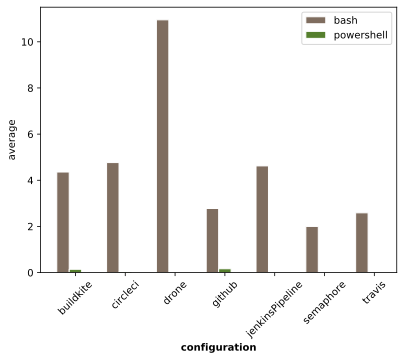
\includegraphics[width=2.5in]{../src/results/scripts usage bars.pdf}
  \caption[alt text]{Mean script usage for each file}
  \label{fig:script_usage}  
\end{figure}



In Table \ref{table:scripts used} we can see the raw count found for each CI service for Bash and Powershell. We were surprised to see the percentages for external scripts to be so high as we expected that use of internal script and functionality that the CI configuration enabled would used relied on more.

\begin{table}
  

\begin{tabular}{|l|l|l|l|l|l|}
\hline
{} &  \multicolumn{2}{c|}{\textbf{bash}} &  \multicolumn{2}{c|}{\textbf{powershell}} & \textbf{total config}\\ \hline
{}                       & count &  percentage usage &  count &  percentage usage & \\ \hline

    % {} &  bash &  powershell &  number of config & percentage bash & percentage powershell \\ \hline
    
    \textbf{Buildkite      } &    61 &    190.62\% &   2  &  6.25\% &    32    \\ \hline
    \textbf{CircleCi       } &  1497 &    134.99\% &   8  &  0.72\% &  1109    \\ \hline
    \textbf{Drone          } &   230 &    273.81\% &   0  &   0.0\% &    84    \\ \hline
    \textbf{Azure          } &     0 &       0.0\% &   0  &   0.0\% &     1    \\ \hline
    \textbf{Github         } &  1097 &     47.67\% &  65  &  2.82\% &  2301    \\ \hline
    \textbf{Jenkins Pipeline} &   171 &    106.21\% &   0  &   0.0\% &    161   \\ \hline
    \textbf{Semaphore      } &     2 &     100.0\% &   0  &   0.0\% &     2    \\ \hline
    \textbf{Teamcity       } &     0 &       0.0\% &   0  &   0.0\% &     4    \\ \hline
    \textbf{Travis         } &  5937 &     55.97\% &   3  &  0.03\% & 10607   \\ \hline

\end{tabular}
\caption{Raw count and percentage chance of each CI service containing an external script}
\label{table:scripts used}
\end{table}

\todo{Add a new conclusion if we are keeping this section}

% As some of the logic is defined in the external scripts and not in the CI file. Potentially there could be less lines of code in the configuration for files that use scripts. However in Figure \ref{fig:script_scatter_lines} we can see that there is little to correlation between script usage and number of lines. Then in Figure \ref{fig:script_scatter_lines2} we can see the same affect when trying to see if the popularity of a project affects the chances of it using CI.
% Falled under this rule: https://twitter.com/daniela_witten/status/1312180956468445186?s=20
% ONE:  CORRELATION DOES NOT IMPLY CAUSATION. 

% Yes, I know you know this, but it’s so easy to forget!

% Yeah, YOU OVER THERE, you with the p-value of 0.0000001 — yes, YOU!! That’s not causation.
% \begin{figure}[!ht]
%   \centering
%   \begin{minipage}[!t]{.48\textwidth}
%     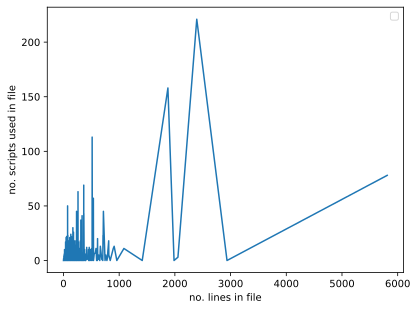
\includegraphics[width=2.5in]{../src/results/scripts vs lines.pdf}
%     \caption{number scripts to number lines with the extreme values cropped out. This shows a slight trend in the more lines you have the more scripts you will use.}
%     \label{fig:script_scatter_lines}    
%   \end{minipage}%
%   \hfill
%   \begin{minipage}[!t]{.48\textwidth}
%     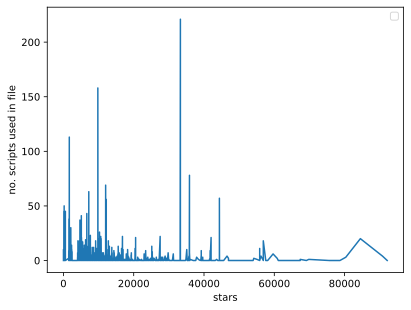
\includegraphics[width=2.5in]{../src/results/scripts vs stars.pdf}
%     \caption{number scripts to stars with the extreme values cropped out. As we are comparing stars along the x axis it looks similar too Figure \ref{graph_scatter_stars_vs_subs}. This figure focuses focused on the first 20,000 stars as that is where the data is most dense. We found a slight increase in usage of scripts the more popular a project became. Yet this is only a correlation and further research would need to be done to work out if their is a causation}
%     \label{fig:script_scatter_lines2}
%   \end{minipage}
% \end{figure}

% Figure \ref{fig:script_scatter_lines} shows the number of lines against the number of scripts used. There is a slight increase in the number scripts used per number of lines. However it is a only very slight increase.

% Figure \ref{fig:script_scatter_lines2} shows that there is no clear correlation between popularity and external script usage. The graph more closely follows the same shape as Figure \ref{graph_scatter_stars_vs_subs}. However much like that other graph there is no clear correlation to be made. Yet there is a clear increase in scripts used after 10,000 stars which is hard to view on the graph. But as the inclusion of a external script is a change because of the amount of potential extra logic added to the configuration file it is significant change. 

% Overall we can see that external scripts are used at least once or more in configuration files. The larger the configuration file their is a slightly higher chance in more external scripts being used. Further research would need to be done to understand at what stage in the CI process they are used. 

\pagebreak

\section{Threats to validating}

The major and most obvious threat is the sample's reliability and validity as it was gathered from scraping the data from GitHub. This has already been touched on in the \ref{methodology} section but now we are going to look at it in more detail critically.

Firstly if we assume that the scraping works perfectly then it only has a maximum of 1000 open source projects per star. That is excluding closed source projects which would range from personal projects to companies. Additionally we only used data from GitHub not from Gitlab, bitbucket or other version control hosting services. This leads to bais in the data for example if Gitlab was also scraped then we would get a lot more Gitlab CI files. However in order to get the best spread of data GitHub has the best API and most of their services do not tie you down to use only their service. Also although we could get a 1000 projects per star we were still able to get around 30,000 projects and a wide spread across GitHub. The key aspect being that because it was a sample we focused on getting a good spread of data.

Secondly, the scraping script is not perfect in how it finds configuration files. This is because it only looks in the top level directory for the file name pattern described in their docs or unique folder. Therefore if the systems allowed many different names or different names in the past it wouldn't have picked it as a CI system. Additionally we only decided to scrape for certain CI files, yet we chose a good scope based on previous research into the top CI files. The scraping script has been tested and worked on to try and minimise any bugs. In the case that we did not pick up a CI file we ran a regexp against the ReadMe file to get a better understanding of the error bounds.

Thirdly, identifying which projects are programming projects or would have a need for CI on GitHub and which are not. Based on the research \cite{Kalliamvakou2014} it is important to filter out repositories that aren't part of the question being asked. Therefore we could have looked to try and filter out GitHub static sites and other none software based projects. However if assume a certain type of project won't be using CI then we would be introducing bais when trying to answer how CI is used. For further research better categorising of projects would help a lot. The major difficulty would be if for example you had a static site that ran on Netlify that will be using CI/CD but very different from a Travis setup. Being able to get the correct data to be able to distinguish and analyse both situations. 


\pagebreak



\section{Summary}

We got a sample of 32,660 open source projects from GitHub and were able to compare that to a previous study 4 years ago. In doing so we found that usage of CI projects was similar and that the more popular a project the higher chance it would be using CI. This linked with the research from 4 years ago. The major change was the increase in the popularity of GitHub Actions, which took over second place from CircleCi. Additionally we looked at whether or not the number of people watching the project had the same effect, it did but to a lesser extent.

% something about the programming table thing we created 

In terms of structure of CI configuration we looked each line of was used in context of comments. We found that a very few projects use comments in their CI. In terms of how they used scripts, we found the majority of projects do not use external scripts. 

From this a better understanding of this topic could be gathered by looking further into the data gathered, as we found we were faced with a lot more questions while doing this research as we go into below.

\vspace*{-0.05in}
\subsection{Discussion and further research}
\vspace*{-0.05in}
In the process of writing this paper we kept on considering more research questions, as there is a lot of meta data that you can get for a single project, in addition to what was used for this paper.

Further research into usage that we would like to do is to look into how the size of the project affects the chance that it uses CI. Then looking at the usage of scripts within CI configuration, for example using a script tag to run a shell script, as while doing the research we found some projects use scripts a lot while others just used the CI configuration. This would lead to questions around which CI system have a higher amount of scripts used, but also looking at how much they enable them to be used and what is the size of those scripts.
The data for the programming language and version(s) is in the configuration. Therefore it would be possible to work out how much usage of a particular programming language each version is getting.

Further research into structure could look into the naming of each part of the build process that is used. This would be interesting as it would provided insight into what terms are commonly used, as well an idea into how people plan or don't plan out their configuration files.
Additionally CI systems can be designed to run on every commit to version control or only commits to certain branches. Therefore by looking at the branching regexp that are being used a better understanding of how branches are actually used in software development where CI is also used could be found out. In particular looking into which branching method (e.g. \cite{BranchGITFLOW2010}, \cite{BranchGITHUBFLOW2017}, \cite{BranchTrunk2013}) is used more for projects with CI and those that don't. 

% In addition working on pruning our dataset using methods outlined in \cite{Kalliamvakou2014}. 

% After looking at these results three areas of research that could be interesting would be filtering the sample to only projects that had recent commits. On the assumption that CI is becoming more popular and stale projects won't require CI.

% Looking into whether or not that assumption is the case. Then looking commit count to see if projects with more commits are more likely to use CI.

\section{Acknowledgement}
We wish to thank Michael Hilton in particular for providing the corpus for their research \citet{Hilton2016}. 

% \appendix
% \section*{Appendix A. Probability Distributions for N-Queens}


\vskip 0.2in
\bibliographystyle{IEEEtran}
\bibliography{sample}


\end{document}
